%%%%%%%%%%%%%%%%%%%%%%%%%%%%%%%%%%%%%%%%%%%%%%%%%%%%%%%%%%%%%%%%%%%%%%
%     File: ExtendedAbstract_resul.tex                               %
%     Tex Master: ExtendedAbstract.tex                               %
%                                                                    %
%     Author: Andre Calado Marta                                     %
%     Last modified : 27 Dez 2011                                    %
%%%%%%%%%%%%%%%%%%%%%%%%%%%%%%%%%%%%%%%%%%%%%%%%%%%%%%%%%%%%%%%%%%%%%%
% Results
% Results should be clear and concise.
% Discussion
% This should explore the significance of the results of the work, not
% repeat them. A combined Results and Discussion section is often
% appropriate. Avoid extensive citations and discussion of published
% literature.
%%%%%%%%%%%%%%%%%%%%%%%%%%%%%%%%%%%%%%%%%%%%%%%%%%%%%%%%%%%%%%%%%%%%%%

\section{Results}
\label{sec:resul}
In this section, the dataset used is described and the results obtained are presented. First, the descriptive statistics are provided, then the DEA scores are obtained, followed by the truncated regression analysis, and finally the Malmquist index results.
\subsection{Dataset description}
\label{subsec:resul_data}
Our dataset includes 41 Iberian airports, including 5 in Portugal and 36 in Spain, over a period of eight years (2016-2023). Following the airport size definition from \cite{ripoll-zarraga2020}, \figref{fig:mapa} displays a map with the geographical location of the airports and their respective sizes.  


\begin{figure}[H]
  \centering
  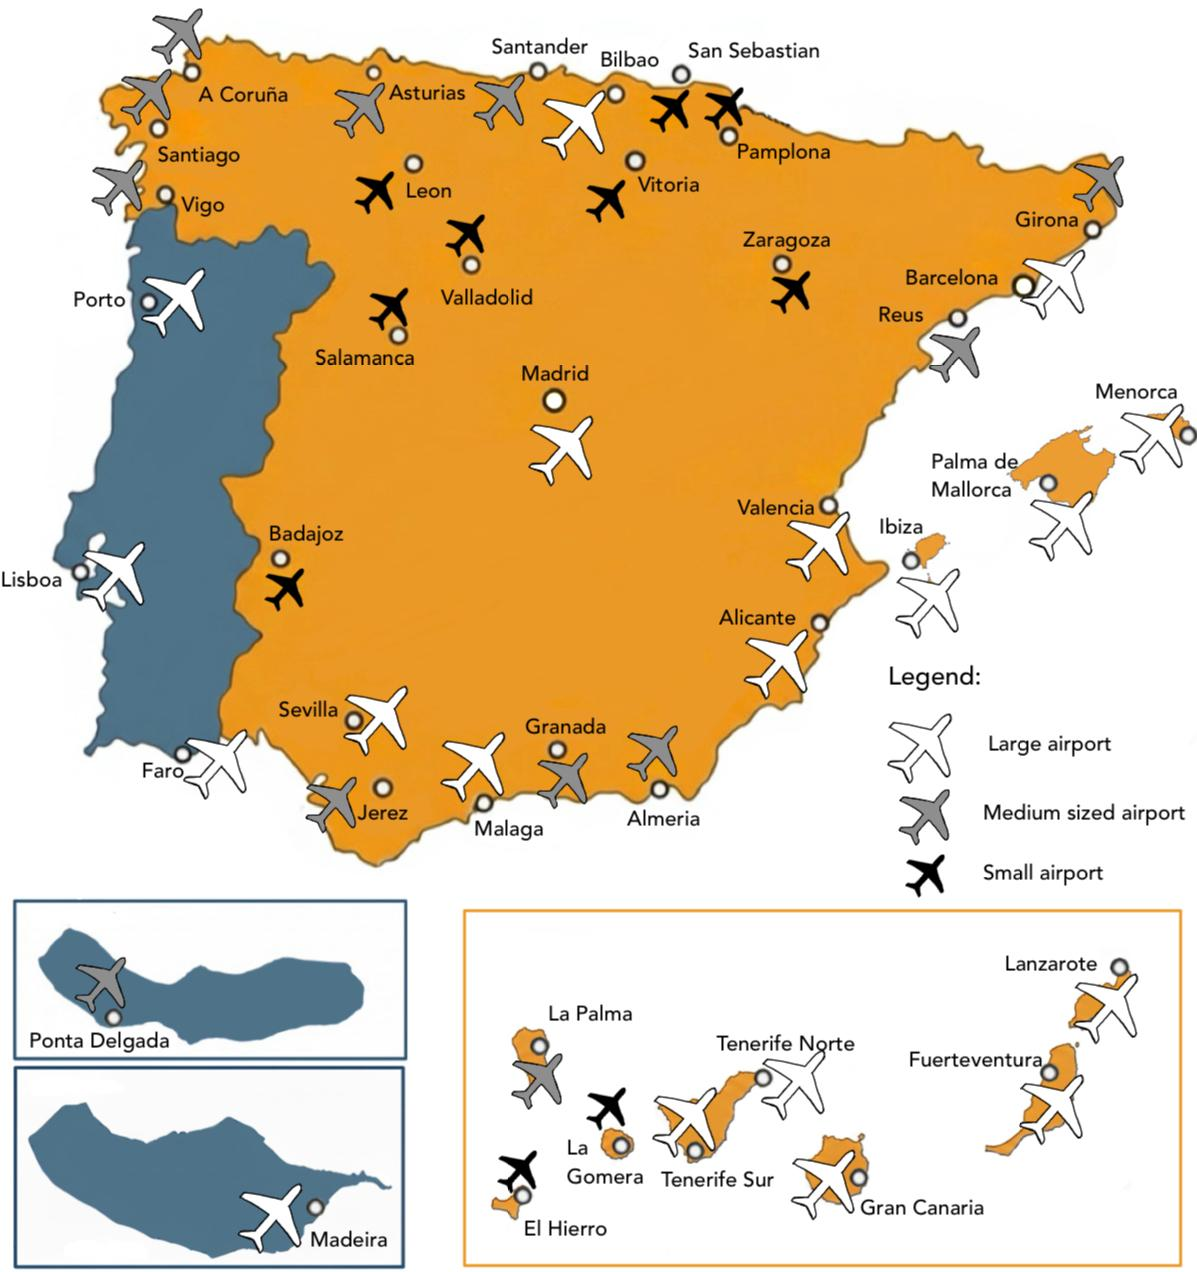
\includegraphics[width=8cm]{images/mapa.jpg}
  \vspace{-0.5cm}
  \caption{Location and size classification of the 41 Iberian airports}
  \label{fig:mapa}
\end{figure}

DEA models require the identification of the inputs and outputs of the analysis. As DEA is not a
statistical technique, there is no systematic approach for the selection of inputs and outputs, therefore the first practical criterion for selecting these
variables is data availability. \tabref{tab:variables} lists these variables
and summarizes their main descriptive statistics, namely the minimum (Min.), maximum (Max.), mean,
and standard deviation (St. Dev.) values.


\begin{table}[h!]
  \begin{center}
    \caption{Summary Statistics for Input and Output Variables (2016–2023)}
    \label{tab:variables}
    \resizebox{\columnwidth}{!}{%
  \begin{tabular}{lcccc}
        \toprule
        \textbf{Variables} & \textbf{Min.} & \textbf{Max.} & \textbf{Mean} & \textbf{St. Dev.} \\
        \midrule
        \multicolumn{5}{l}{\textit{Inputs}} \\
       Employees & 17 & 42,222 & 3,409 & 7,862 \\
         Runway \\Area
    ($m^2$) & 37,500 & 910,020 & 169,293 & 142,191 \\
        Gates & 2 & 238 & 24.8 & 42.4 \\
        \midrule
        \multicolumn{5}{l}{\textit{Outputs}} \\
         Passengers & 2,358 & 61,652,021 & 6,437,865 & 11,112,114 \\
        ATM & 1,086 & 426,324 & 53,780 & 76,780 \\
         Cargo (t) & 0 & 655,586 & 27,546 & 89,429 \\
        \bottomrule
 \end{tabular}%
    }
  \end{center}
\end{table}
  
Even though this selection of input variables does not fully
represent the most common variables in the literature review conducted in \autoref{sec:backg} due to data availability constraints, it is still in line with the previous literature.

It is important to highlight that only physical measures of capital were considered in this analysis. This
approach was necessary since airport-level financial data stopped being published, following Aena’s partial privatization in 2014.

Regarding the second-stage regression, \tabref{tab:exp_statistics} lists the explanatory variables used in the second-stage regression to explain DEA efficiency scores.


\begin{table}[h!]
  \begin{center}
        \caption{Summary Statistics for explanatory variables}
    \label{tab:exp_statistics}
    % Define centered column type
   \resizebox{\columnwidth}{!}{%
  \begin{tabular}{lcccc}
        \toprule
        \textbf{Explanatory Variables} & \textbf{Min.} & \textbf{Max.} & \textbf{Mean} & \textbf{St. Dev.} \\
        \midrule
        Island & 0 & 1 & 0.32 & 0.47 \\
        Military & 0 & 1 & 0.27 & 0.44 \\
        Rail existence & 0 & 1 & 0.10 & 0.30 \\
        Share of cargo (\%) & 0 & 89.33 & 4.68 & 15.65 \\
        Share of LCC passengers (\%) & 0 & 96.67 & 49.62 & 26.78 \\
        \bottomrule
  \end{tabular}%
    }
  \end{center}
\end{table}
  
Island is a binary variable indicating whether an airport is located on an island (Island=1) or the
mainland (Mainland=0). The inclusion of this variable is justified, as 13 out of the 49 airports in the
dataset operate on an island. Military is another binary variable indicating whether there are military
operations at the airport. In the considered dataset, 11 out of the 41 airports operate as mixed civil-military airports.
Share of cargo represents the percentage of cargo in the total WLU and Share of LCC passengers represents the percentage of low-cost carrier (LCC) passengers in the total
number of passengers. Due to data constraints from the Portuguese airports, only the passengers from
LCCs ranked among the top 10 airlines at each airport (by passenger volume) are considered.
Additionally, a novel input in Iberian airport efficiency studies was included: the existence of a railway connection inside the airport. This variable was included to capture the impact of intermodal connectivity on airport efficiency.







\subsection{First-stage: Static DEA scores}
\label{subsec:resul_dea}  
The first stage of the analysis involved calculating the efficiency scores for each airport across the
different years considered. For that, an output oriented DEA model under Variable Returns to Scale
(VRS) was applied.

The choice of output orientation is particularly appropriate in the context of Iberian airports, since
most of the Spanish airports operate with overcapacity, meaning the existing infrastructure is underutilized \cite{nerja2021}. As some of the airport inputs are considered fixed in the short and medium term, airport managers have limited capacity to adjust input levels,
and should, therefore, focus on maximizing their utilization \cite{martin2001}. Regarding the returns to scale, VRS was assumed due to the large size difference between the airports considered, as shown in \figref{fig:mapa}. Nonetheless, the CRS
scores were also determined for the calculation of Scale efficiencies. 

\tabref{tab:crs,vrs,scale} presents the bootstrapped results obtained for each airport. It includes the average efficiency scores for Constant Returns to Scale (CRS), Variable Returns to Scale (VRS), and Scale efficiency (Scale) for each airport. It should be noted that the biased scores were also calculated for comparison, even though they are not presented here for brevity. Following the definition in \eqnref{eq:rts_definition}, the last column indicates the type of returns to scale (RTS) each airport is operating, which can
be either Increasing Returns to Scale (IRS), Decreasing Returns to Scale (DRS), or Constant Returns to Scale (CRS). As this study analyzes a period of 8 years, different classifications can be obtained in
different years. In \tabref{tab:crs,vrs,scale}, the most common classification will be displayed. In cases where the two
most common classifications are observed the same number of times across the eight-year period, both
classifications are presented.

\renewcommand{\arraystretch}{0.9}
\begin{table}[t!]
\centering
\caption{Bootstrapped average CRS, VRS and Scale efficiencies.} 
\vspace{0.1cm}
\label{tab:crs,vrs,scale}
\resizebox{\columnwidth}{!}{%
\begin{tabular}{lcccc}
  \toprule
  \textbf{Airports} & \textbf{CRS} & \textbf{VRS} & \textbf{Scale} & \textbf{RTS}  \\
  \midrule

% no \endhead here to prevent repeated header

% === Table rows start here ===
A Coruña & 0.323 & 0.343 & 0.941 & IRS\\
A S Madrid-Barajas & 0.568 & 0.823 & 0.693 & DRS\\
Alicante & 0.591 & 0.596 & 0.988 & IRS/DRS \\
Almeria & 0.226 & 0.232 & 0.978 & IRS/CRS\\
Asturias & 0.188 & 0.190 & 0.987 & CRS\\
Badajoz & 0.121 & 0.360 & 0.335 & IRS\\
Barcelona & 0.382 & 0.741 & 0.518 & DRS\\
Bilbao & 0.436 & 0.501 & 0.871 & DRS\\
El Hierro & 0.325 & 0.768 & 0.425 & IRS\\
Faro & 0.514 & 0.551 & 0.928 & IRS\\
FGL Granada & 0.366 & 0.414 & 0.883 & IRS\\
Fuerteventura & 0.353 & 0.370 & 0.952 & DRS\\
Girona & 0.183 & 0.186 & 0.982 & IRS/CRS\\
Gran Canaria & 0.448 & 0.552 & 0.809 & IRS\\
Ibiza & 0.694 & 0.698 & 0.991 & DRS/CRS\\
Jerez & 0.653 & 0.680 & 0.961 & DRS\\
La Gomera & 0.183 & 0.516 & 0.388 & IRS\\
La Palma & 0.276 & 0.288 & 0.959 & IRS\\
Lanzarote & 0.588 & 0.596 & 0.985 & IRS\\
Leon & 0.124 & 0.492 & 0.297 & IRS\\
Lisbon & 0.617 & 0.701 & 0.880 & IRS\\
Madeira & 0.237 & 0.254 & 0.933 & IRS\\
Malaga & 0.522 & 0.583 & 0.883 & DRS\\
Menorca & 0.332 & 0.342 & 0.970 & IRS/DRS\\
Palma De Mallorca & 0.464 & 0.661 & 0.701 & IRS\\
Pamplona & 0.173 & 0.224 & 0.776 & IRS\\
Ponta Delgada & 0.417 & 0.703 & 0.596 & IRS\\
Porto & 0.608 & 0.650 & 0.923 & IRS\\
Reus & 0.262 & 0.262 & 0.999 & IRS/CRS\\
Salamanca & 0.645 & 0.649 & 0.995 & IRS/CRS\\
San Sebastian & 0.128 & 0.148 & 0.866 & IRS\\
Santiago & 0.234 & 0.243 & 0.963 & DRS\\
Santander & 0.191 & 0.193 & 0.992 & CRS\\
Sevilla & 0.534 & 0.564 & 0.946 & DRS\\
Tenerife-Norte & 0.534 & 0.580 & 0.916 & IRS\\
Tenerife-Sur & 0.636 & 0.658 & 0.966 & DRS\\
Valencia & 0.536 & 0.550 & 0.971 & IRS\\
Valladolid & 0.177 & 0.178 & 0.995 & CRS\\
Vigo & 0.168 & 0.168 & 0.997 & CRS\\
Vitoria & 0.563 & 0.694 & 0.820 & IRS\\
Zaragoza & 0.802 & 0.822 & 0.976 & IRS\\
\midrule
Mean & 0.398 & 0.480 & 0.854 & \\
Mean excluding COVID & 0.436 & 0.522 & 0.859 & \\
\# of efficient DMUs & 0 & 0 & 18 & \\
\bottomrule
\end{tabular}%
}
\end{table}
Analyzing \tabref{tab:crs,vrs,scale}, it is possible to observe that Iberian airports present low values of efficiency,
averaging 0.480 for the bootstrapped VRS model, in the years under
analysis.
When excluding the years 2020 and 2021, due to the COVID-19 pandemic, the average
bootstrapped VRS efficiency increases to 0.522, while the CRS model increases to 0.436. It is also
possible to note that there is no average efficiency score of 1, with a maximum observed
value of 0.823 for Madrid-Barajas airport, meaning none of the considered airports operates in the
frontier. Regarding scale efficiency, the average bootstrapped scale efficiency is 0.854, indicating that
Iberian airports are not operating at their optimal scale.


\subsection{Second-stage: Truncated regression }
\label{subsec:resul_trunc}

After computing the DEA efficiency scores in the first stage, a second-stage truncated regression
was conducted to address DEA’s main limitation, which is its inability to explain the effect of some
determinants in the efficiency scores. The regression was applied to the bootstrapped DEA scores, using the explanatory variables described in \tabref{tab:exp_statistics}, under the following model:


\begin{equation}
    \label{eq:complete_regression}
\begin{aligned}
\theta_{i,t} &= \alpha + \beta_1 \text{Island}_{i} + \beta_2 \text{Military}_{i} + \beta_3 \text{Rail}_{i} \\
&\quad + \beta_4 \text{ShareCargo}_{i,t} + \beta_5 \text{ShareLCC}_{i,t} + \varepsilon_{i,t}
\end{aligned}
\end{equation}

reports the coefficients and p-values for the variables considered in both the biased and
bootstrapped models. For binary variables, the coefficient represents the estimated change in the effi-
ciency score when the specific variable applies, while for continuous variables, the coefficient reflects
the marginal effect on the efficiency score of a one-unit increase in the corresponding variable \cite{simar2007}.


\subsection{Dynamic Evolution: Malmquist index}
\label{subsec:resul_malm}





%%%%%%%%%%%%%%%%%%%%%%%%%%%%%%%%%%%%%%%%%%%%%%%%%%%%%%%%%%%%%%%%%%%%%%

%\begin{table}[!h]
 %\begin{center}
  %  \begin{tabular}{lccc}
   %   Model           & $C_L$ & $C_D$ & $C_{M y}$ \\
    %  \hline
  %    Euler           & 0.083 & 61,652,021  & -0.110    \\
   %   Navier--Stokes  & 0.078 & 0.023 & -0.101    \\
    %  \hline
    %\end{tabular}
  %\end{center}
  %\caption[Table caption shown in TOC]{Table caption}
  %\label{table:simple}
%\end{table}
